% results.tex
% Results section of the manuscript
% Stephan Gahima/paper-draft-tex

\section{Results \label{sec:results}}
	
	To visualize the sparsity pattern of a matrix \(\mat{S}\in\mathbb{R}^{100\times 100}\) and the classification of the \href{https://en.wikipedia.org/wiki/Iris_flower_data_set}{Fisher's iris dataset}, you can use the Matlab source codes \ref{code:fig2a}-\ref{code:fig2b}. Running these codes will produce the output \reffig{fig:math-stuff}.
	
	\begin{lstlisting}[style=Matlab-editor, caption={Matlab code for \reffig{fig:sparsity}}, label=code:fig2a]
		 S = sprand(100,100,0.1);
		 spy(S);
	\end{lstlisting}
		
	\begin{lstlisting}[style=Matlab-editor, caption={Matlab code for \reffig{fig:classification}}, label=code:fig2b]
		load fisheriris.mat; 
		gscatter(meas(:,1),meas(:,2),species,'rgb', 'osd');
		xlabel('Sepal length');
		ylabel('Sepal width');
	\end{lstlisting}
	
	To correctly size figures without rescaling, you need to know the \verb*|\textwidth| and  \verb*|\textheight| LaTex is using. 
	% Ref. https://tex.stackexchange.com/questions/39383/determine-text-width
	To do so, add the \verb*|layourts| package (here is already included!) and \verb*|\printinunitsof{cm}\prntlen{\textwidth}| (or \verb*|\printinunitsof{cm}\prntlen{\textheight}|) gives \verb*|\textwidth| = \printinunitsof{cm}\prntlen{\textwidth} (or \verb*|\textheight| = \printinunitsof{cm}\prntlen{\textheight}).
	% For inches, use \printinunitsof{in}\prntlen{\textwidth}
	This information is an input for \verb*|ffsp|: a Matlab function written to nicely format figures. 
	For instance, to produce \reffig{fig:math-stuff} we added \verb*|ffsp(gcf,gca,17.5875,22.93674,1,2)| to both source codes \ref{code:fig2a}-\ref{code:fig2b}.
	In \refapp{sec:ffsp}, we explain how \verb*|ffsp| works.
	
	% https://latex-tutorial.com/subfigure-latex/ to know more about the SUBFIGURE environment
	\begin{figure}[H]
		\centering
		\begin{subfigure}[b]{\twofig\textwidth} 
			% Add reference to the code that produced the figure
			\includegraphics{fig/spy.pdf}
			\subcaption{
				Sparsity pattern of matrix \(\mat{S}\).
				\label{fig:sparsity}
			}
		\end{subfigure}
		\hfil
		\begin{subfigure}[b]{\twofig\textwidth}
			% Add reference to the code that produced the figure
			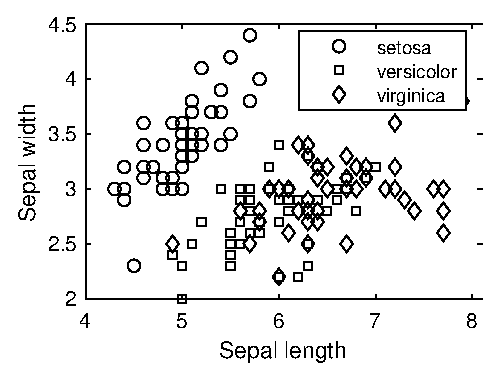
\includegraphics{fig/gscatter.eps}
			\subcaption{
				Classification of the Fisher's iris dataset.
				\label{fig:classification}
			}
		\end{subfigure}
		\caption{PDF (a) and EPS (b) generated figures. \label{fig:math-stuff}}
	\end{figure}